%================================================================
\section{Introduction}

Interactive digital storytelling has traditionally been concerned with
text-based modes of discourse. Despite the fact that the word {\em fiction}
makes no commitments to medium (book, film, play, et cetera), the term {\em
interactive fiction} is used nearly synonymously with text-based digital
storytelling. Meanwhile, comics, a relatively unexplored domain of
computational narratology~\cite{mani2012computational}, present a wide
range of expressive opportunities for interactive storytelling not afforded
by text.  Interactive comics invite many of the same questions addressed by
interactive textual narrative research: what modes are available for a
machine to tell visual stories in collaboration with a human player or
author? How can algorithms introduce novel, generative content into a
partially-constructed comic?  Which decisions will the human and
algorithmic components have available to them?

This work begins to address these questions by exploring generation of {\em
purely visual}, {\em abstract} comics. ``Purely visual'' means that panels
do not use words and text to communicate narrative, as in
Figure~\ref{fig:calvin}. ``Abstract,'' as in abstract art, means that,
aside from repetition of elements with a shape, color, and size, and
spatial placement of said entities within panels, we do not intentionally
ascribe literal meaning to the components of generated panels. Our purpose
in choosing an abstract representation is partially due to ease of
implementation, but partially also to separate issues of {\em structure} of
comics (which can be perceived with abstract representations) from issues
of contextual, reference-laden meaning that would be found especially in
anthropomorphic figures. (XXX cite)

% While most approaches to text generation in the tradition of interactive
% storytelling research has focused on a ``pipeline
% model''~\cite{ronfard2014story}, first generating a plot structure and then
% developing a discourse after the fact, this is not the only
% available nor most suitable approach for visual narrative. 

Two leading theories on comics have examined constraints on sequences of panels
and the relationships among them.
McCloud~\cite{mcCloud1993understanding} proposes a taxonomy of {\em
transitions} between a panel and the one following it, enumerating six
different ways readers might make sense of the connection between two
consecutive panels ``across the gutter'' (gap between panels).
Cohn~\cite{cohn2013visual}, on the other hand, eschews transitions as a
basis for comic structure and asserts that grammar-like syntax trees govern
the formation of legible comics.
We present a small-scale computational
system~\cite{montfort2012small} that operationalizes a hybrid of these two
approaches.


\begin{figure}
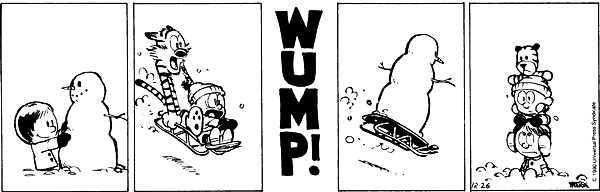
\includegraphics[width=\columnwidth]{calvin-and-hobbes.png}
\caption{
This wordless Calvin and Hobbes comic strip ({\small \copyright}~Bill Watterson)
exemplifies the kind of output we are targeting with our generator. The strip also
illustrates how little plot structure informs this kind of short-form visual
storytelling.
}
\label{fig:calvin}
\end{figure}

In the remainder of this paper, we discuss theoretical aspects of comics
authoring, our computational implementation of a comic generation system,
and our experience with refining our model with linguistic constraints. Our
primary takeaway is that both {\em global and local} reasoning contribute
important techniques to narrative generation: local reasoning is important for
maintaining narrative coherence, and global reasoning is important for
maintaining satisfying narrative structure. Both are thus important parts
of creating comprehensible comics, and we present an outline of future work
designed to explore the human interpretation of our generated artifacts.

